\small
Over the last decade, Python grew a vast and rich ecosystem of scientific third
party libraries. \textbf{ObsPy serves as a bridge} and enables its users to
effortlessly tie into this system giving access to large amounts of tools
designed to process and analyze data. This box quickly introduces the core
packages needed for scientific analysis.

\vspace{1ex}
\noindent\hrulefill
\vspace{1ex}

    \begin{center}
    \begin{tabularx}{\textwidth}{rX}
        \begin{minipage}{0.25\columnwidth}
            \begin{center}
            
\includegraphics[height=4cm]{./images/ipython.png}
            \end{center}
        \end{minipage}
        &
        \begin{minipage}{0.7\columnwidth}
            \textbf{IPython:} Enhanced Interactive Console
            \vspace{0.5ex}
            \footnotesize{
                \begin{itemize}
                    \item Powerful interactive shells (terminal and Qt-based)
                    \item A browser-based notebook with support for code, text, mathematical expressions, inline plots and other rich media
                    \item Easy to use, high performance tools for parallel computing
                \end{itemize}
            }

        \end{minipage}
    \end{tabularx}
    \end{center}

\vspace{1ex}
\noindent\hrulefill
\vspace{1ex}

    \begin{center}
    \begin{tabularx}{\textwidth}{rX}
        \begin{minipage}{0.25\columnwidth}
            \begin{center}
            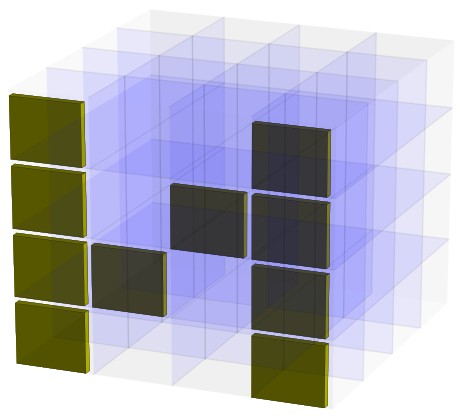
\includegraphics[height=4cm]{./images/numpy_logo.png}
            \end{center}
        \end{minipage}
        &
        \begin{minipage}{0.7\columnwidth}
            \textbf{NumPy:} \textit{Modern Array Processing}
            \vspace{0.5ex}

            \footnotesize{NumPy is the fundamental package needed for scientific
                computing with Python. Besides its obvious scientific uses, NumPy
                can also be used as an efficient multi-dimensional container of generic
                data. Arbitrary data-types can be defined. This allows NumPy to seamlessly
                and speedily integrate with a wide variety of databases.}
        \end{minipage}
    \end{tabularx}
    \end{center}

%\vspace{1ex}
%\noindent\hrulefill
%\vspace{1ex}
\columnbreak


    \begin{center}
    \begin{tabularx}{\textwidth}{rX}
        \begin{minipage}{0.25\columnwidth}
            \begin{center}
            
\includegraphics[height=4cm]{./images/scipy_med.png}
            \end{center}
        \end{minipage}
        &
        \begin{minipage}{0.7\columnwidth}
            \textbf{SciPy:} \textit{Fundamental library for scientific computing}
            \vspace{0.5ex}

            \footnotesize{SciPy is open-source software for mathematics,
                science, and engineering. It is also the name of a very popular
                conference on scientific programming with Python. The SciPy
                library depends on NumPy, which provides convenient and fast
                N-dimensional array manipulation. The SciPy library is built to
                work with NumPy arrays, and provides many user-friendly and
                efficient numerical routines such as routines for numerical
            integration and optimization.}

        \end{minipage}
    \end{tabularx}
    \end{center}

\vspace{1ex}
\noindent\hrulefill
\vspace{1ex}

    \begin{center}
    \begin{tabularx}{\textwidth}{rX}
        \begin{minipage}{0.25\columnwidth}
            \begin{center}
            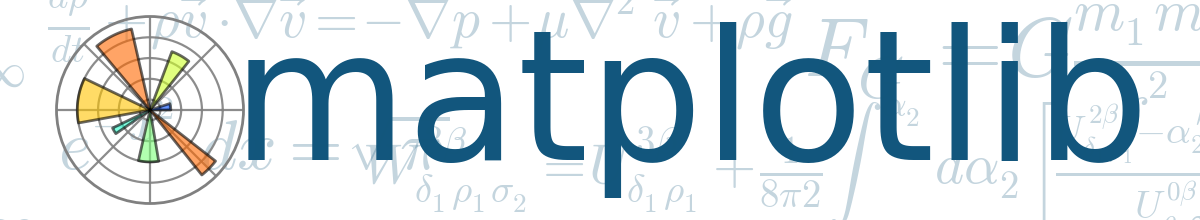
\includegraphics[width=6cm]{./images/matplotlib_med.png}
            \end{center}
        \end{minipage}
        &
        \begin{minipage}{0.7\columnwidth}
            \textbf{Matplotlib:} \textit{Comprehensive, high quality 2D Plotting}
            \vspace{0.5ex}

            \footnotesize{2D plotting library for Python that produces high
                quality figures that can be used in various hardcopy and
                interactive environments.}
        \end{minipage}
    \end{tabularx}
    \end{center}

\vspace{1ex}
\noindent\hrulefill
\vspace{1ex}

    \begin{center}
    \begin{tabularx}{\textwidth}{rX}
        \begin{minipage}{0.25\columnwidth}
            \begin{center}
            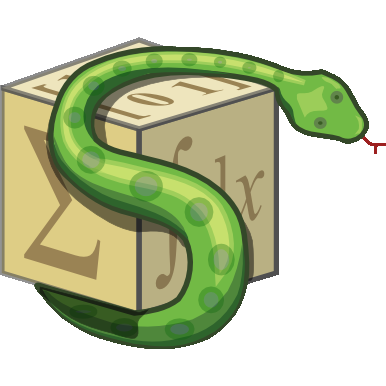
\includegraphics[height=4cm]{./images/sympy_logo.png}
            \end{center}
        \end{minipage}
        &
        \begin{minipage}{0.7\columnwidth}
            \textbf{SymPy:} \textit{Symbolic mathematics}
            \vspace{0.5ex}

            \footnotesize{SymPy is a Python library for symbolic mathematics.
                It aims to become a full-featured computer algebra system (CAS)
                while keeping the code as simple as possible in order to be
                comprehensible and easily extensible. SymPy is written entirely
                in Python and does not require any external libraries.}
        \end{minipage}
    \end{tabularx}
    \end{center}

%\vspace{1ex}
%\noindent\hrulefill
%\vspace{1ex}
\columnbreak

    \begin{center}
    \begin{tabularx}{\textwidth}{rX}
        \begin{minipage}{0.25\columnwidth}
            \begin{center}
            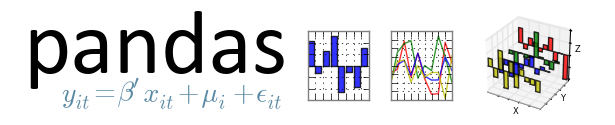
\includegraphics[width=6cm]{./images/pandas.png}
            \end{center}
        \end{minipage}
        &
        \begin{minipage}{0.7\columnwidth}
            \textbf{pandas:} \textit{Data structure \& analysis}
            \vspace{0.5ex}

            \footnotesize{pandas is a Python package providing fast, flexible, and expressive data structures designed to make working with “relational” or “labeled” data both easy and intuitive. It aims to be the fundamental high-level building block for doing practical, real world data analysis in Python. Additionally, it has the broader goal of becoming the most powerful and flexible open source data analysis / manipulation tool available in any language.}
        \end{minipage}
    \end{tabularx}
    \end{center}


\vspace{1ex}
\noindent\hrulefill
\vspace{1ex}

    \begin{center}
    \begin{tabularx}{\textwidth}{rX}
        \begin{minipage}{0.25\columnwidth}
            \begin{center}
            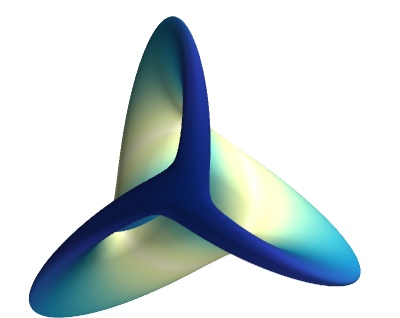
\includegraphics[width=6cm]{./images/mayavi.png}
            \end{center}
        \end{minipage}
        &
        \begin{minipage}{0.7\columnwidth}
            \textbf{Mayavi:} \textit{3D Scientific Data Visualization and Plotting}
            \vspace{0.5ex}

            \footnotesize{
                \begin{itemize}
                    \item A simple and clean scripting interface in Python, including one-liners, or an object-oriented programming interface. Mayavi integrates seamlessly with numpy and scipy for 3D plotting and can even be used in IPython interactively, similarly to Matplotlib.
                    \item The power of the VTK toolkit, harnessed through these interfaces, without forcing you to learn it.
                \end{itemize}

            }
        \end{minipage}
    \end{tabularx}
    \end{center}
